\subsection{Анализ опасных и вредных факторов при разработке}

\subsubsection{Введение}

В рамках данного дипломного проекта проводится проектирование системы управления
манипулятора, расположенного на борту спутника, на основе шагового привода.
Основным рабочим местом является стол, оборудованный персональной ЭВМ
(далее --- ПЭВМ) с визуально~--~дисплейным терминалом (далее --- ВДТ) и макетом
манипулятора, который состоит из платы управления, экспериментального стенда с
имитацией нагрузочных моментов, внешнего источника питания и шагового двигателя
(рис. (\ref{pic_workplace_scheme})).

Помимо специфических условий зрительной работы, напряженного
нервно~--~эмоционального характера труда, вынужденной рабочей позы, недостатка
подвижности и физической активности, работающие за ВДТ подвергаются воздействию
низкоэнергетического УФ и рентгеновского излучений, шума, электромагнитных и
электростатических полей, неудовлетворительного микроклимата, вентиляции и
освещения.

\subsubsection{Характеристики рабочих помещений}

Согласно СанПиН 2.2.2/2.4.1340--03 \cite{ecology_sanpin_1340_03}, площадь на одно
рабочее место с ВДТ и ПЭВМ должна составлять не менее 6--ти $\text{м}^2$, а объем
--- не менее 20--ти $\text{м}^3$. Расстояние между тыльной частью одного видеомонитора
и экраном другого видеомонитора должно быть не менее 2--х метров, а расстояние
между их боковыми поверхностями --- не менее 1.2--х м. Схема рабочего помещения
изображена на рис (\ref{pic_workroom_scheme}).

\begin{figure}[ht!]
    \centering
    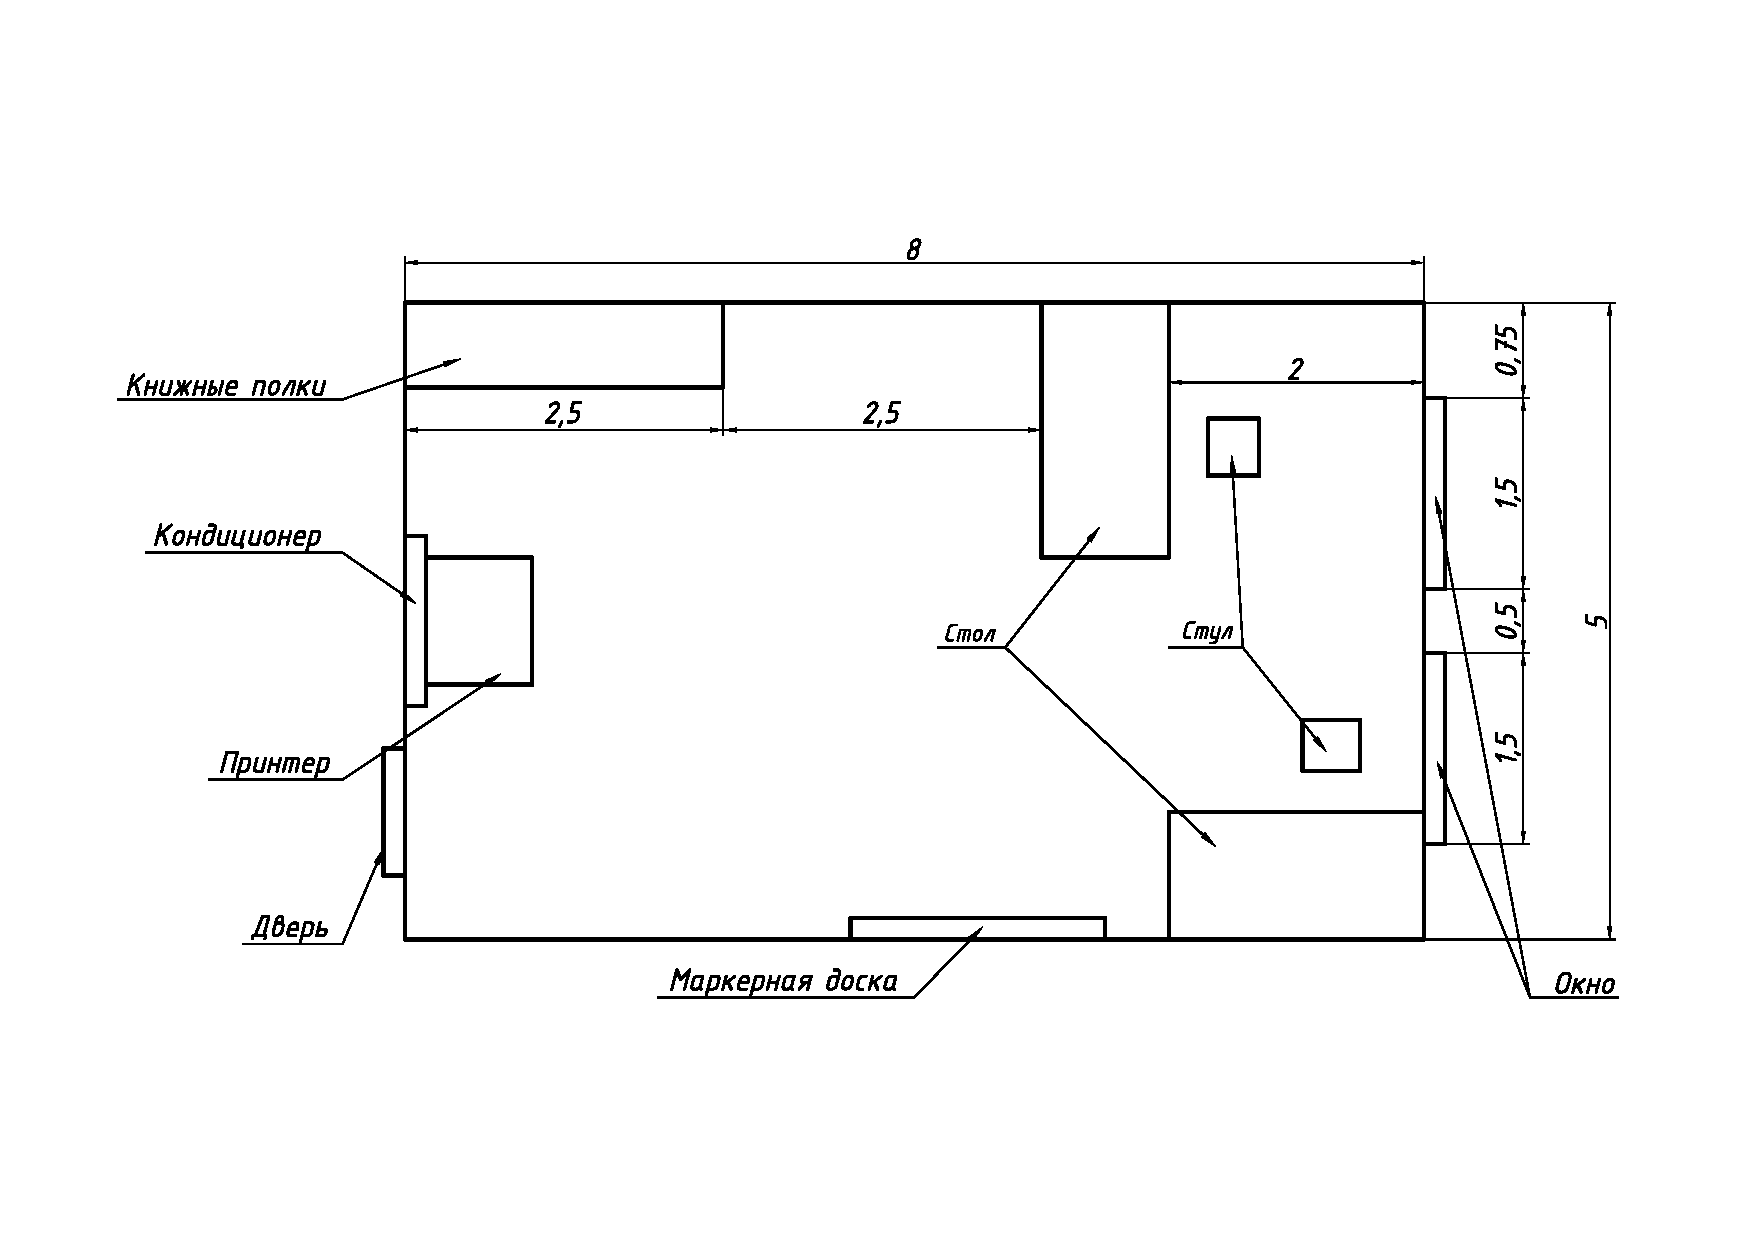
\includegraphics[width=\textwidth, keepaspectratio, clip=true, trim=0mm 35mm 0mm 35mm]
                    {./src/ecology/pictures/workroom_scheme}
    \caption{Схема рабочего помещения (размеры в метрах)}
    \label{pic_workroom_scheme}
\end{figure}

Согласно СанПиН 2.2.2/2.4.1340--03 \cite{ecology_sanpin_1340_03}, помещения с ВДТ
и ПЭВМ должны иметь естественное и искусственное освещение. Рабочее место по
отношению к световым проёмам должно располагаться так, чтобы естественный свет
падал сбоку, преимущественно слева. Необходимо обеспечивать коэффициент
естественной освещенности (КЕО) не ниже $1.2 \%$ в зонах с устойчивым снежным
покровом и не ниже $1.5 \%$ на остальной территории.
Для обеспечения этих требований произведён соответствующий расчёт в разделе
\ref{lighting_calculation}. Геометрия расположения светильников изображена на рис.
(\ref{pic_lamps_arrangement}).

Рабочее помещение не граничит с помещениями, в которых уровни шума и вибрации превышают
нормируемые значения. Звукоизоляция ограждающих конструкций помещений с ВДТ и ПЭВМ
отвечает гигиеническим требованиям и обеспечивает нормируемые параметры шума
согласно требованиям санитарных норм 2.2.4./2.1.8.562--96 \cite{ecology_sanitary_norm_562_96}.

Для обеспечения требований к микроклимату рабочего помещения по СанПин 2.2.4.548--96
\cite{ecology_sanpin_548_96} используется оборудоваться системами отопления,
кондиционирования воздуха.

Для обеспечения допустимых параметров воздуха, в рабочем помещении используется
приточно~--~вытяжная система вентиялции.

Для внутренней отделки интерьера помещений с ВДТ и ПЭВМ используются
диффузно~--~отражающие материалы с коэффициентом отражения $0.7 - 0.8$ для потолка,
$0.5 - 0.6$ для стен, $0.3 - 0.5$ для пола. Полимерные материалы, используемые для
внутренней отделки интерьера помещений с ВДТ и ПЭВМ, разрешены для применения
органами и учреждениями Государственного Санитарно~--~Эпидемиологического
Надзора.

Для подвода питания к электрооборудованию в помещении используются розетки,
подключенные к трёхфазной пятипроводной сети переменного тока с глухим
заземлением нейтрали и автоматами защиты от перегрузок. Напряжение сети
составляет 220 В, частота 50 Гц.

Рабочее место организовано следующим образом:
\begin{itemize}
    \item   Высота над уровнем пола рабочей поверхности, за которой работает
            инженер~--~программист, составляет 72 см
    \item   Размеры поверхности стола 2 м $\cdot$ 1 м
    \item   Под столом предстусмотрено пространство для ног с глубиной в 65 см
    \item   Рабочий стул разработчика снабжен подъемно--поворотным механизмом; высота
            сиденья регулируется в пределах 50 cм; глубина сиденья должна составляет
            не менее 38--ми cм, а ширина --- не менее 40 cм;
            высота опорной поверхности спинки --- не менее 30--ти cм, ширина – не
            менее 38--ми см; угол наклона спинки стула к плоскости сиденья
            изменяется в пределах $90 \degree$
    \item   Экран монитора находиться от глаз пользователя на оптимальном
            расстоянии $0.6 - 0.7$ м, но не ближе 0,5 м с учетом размеров
            алфавитно~--~цифровых знаков и символов
\end{itemize}

Схема рабочего места показаны на рис. (\ref{pic_workplace_scheme}), где \\
1 -- Стол                \\
2 -- Макет манипулятора  \\
3 -- ПЭВМ                \\
4 -- ВДТ                 \\
5 -- Клавиатура          \\
6 -- Стул

\begin{figure}[ht!]
    \centering
    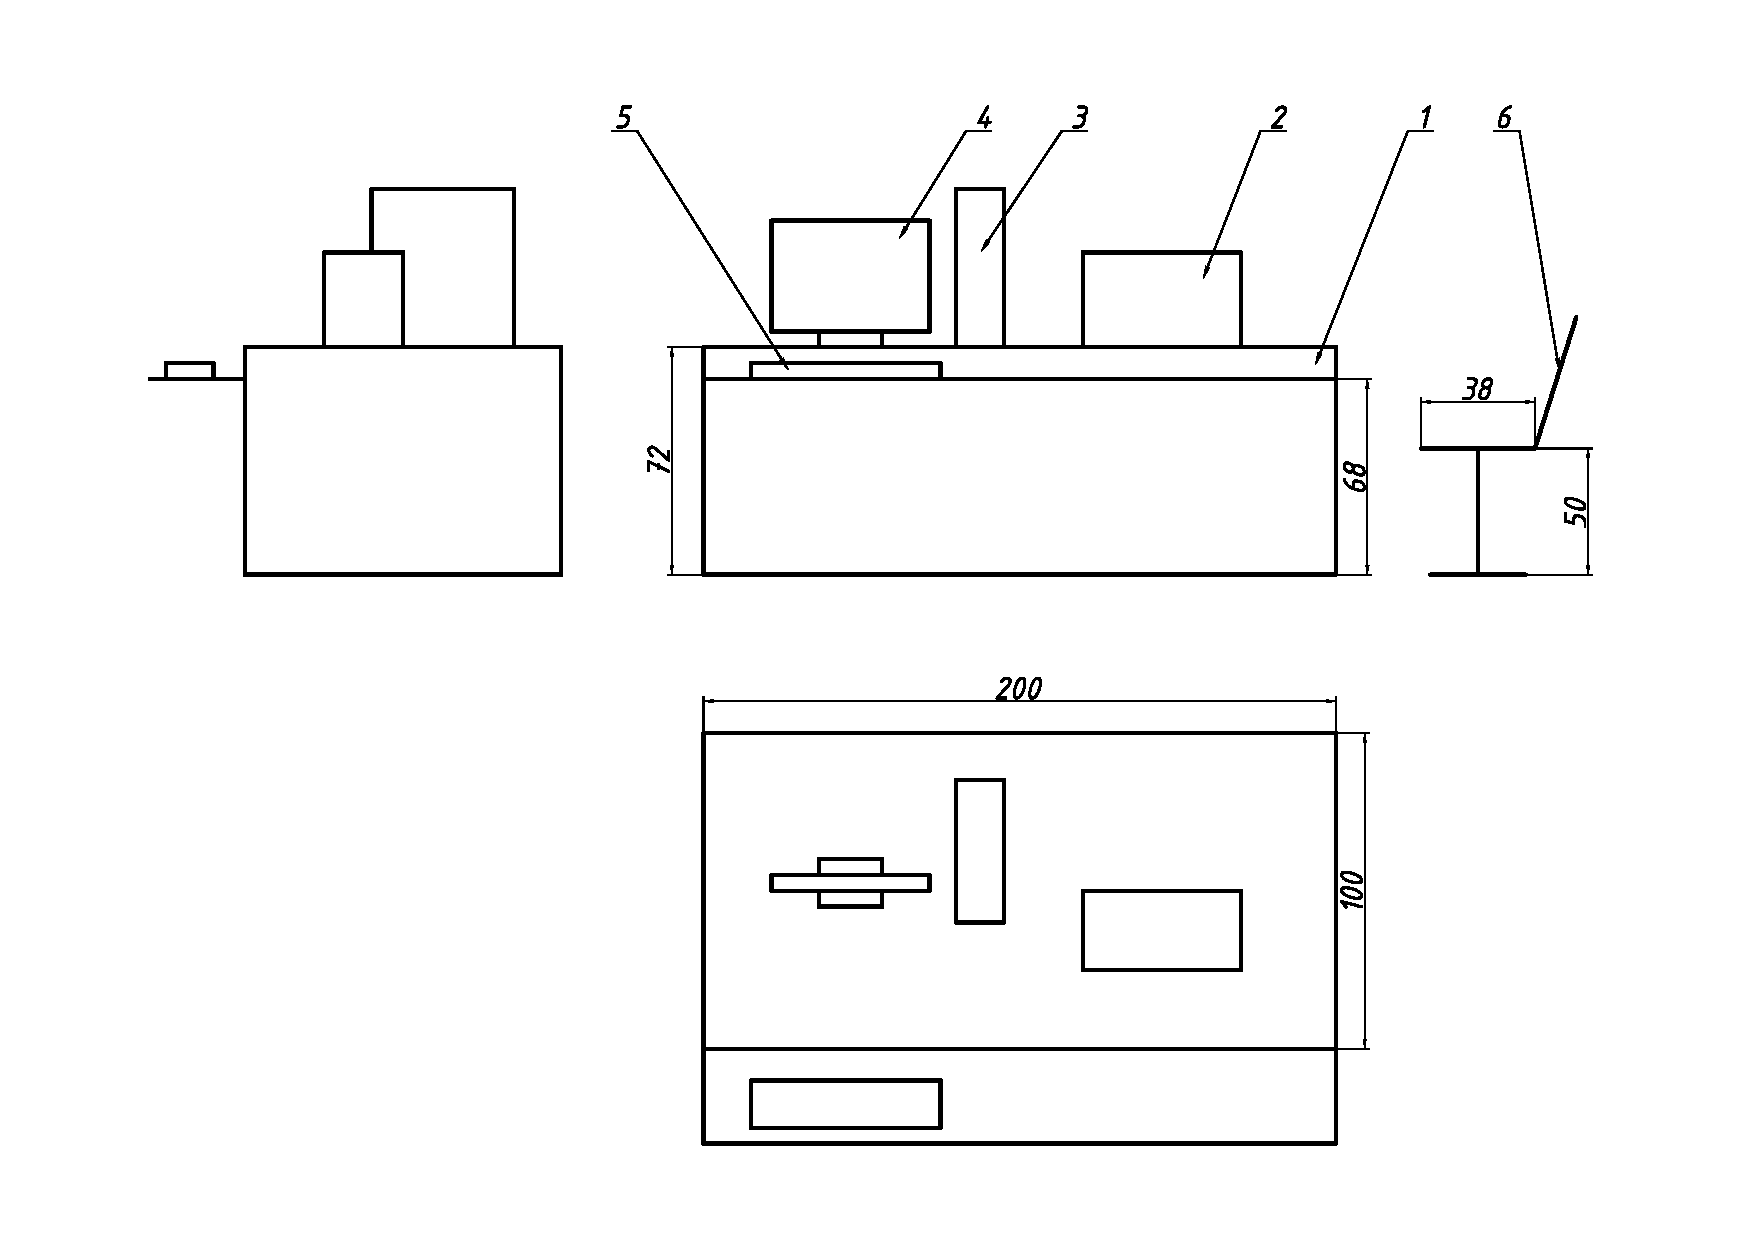
\includegraphics[width=\textwidth, keepaspectratio, clip=true, trim=0mm 10mm 0mm 15mm]
                    {./src/ecology/pictures/workplace_scheme}
    \caption{Схема рабочего места (размеры в сантиметрах)}
    \label{pic_workplace_scheme}
\end{figure}

Для снижения отрицательного воздействия излучений от компьютера
на здоровье работника, предусмотрен режим труда и отдыха в зависимости от выполняемой
работы и возраста пользователя. Независимо от вида выполняемой работы, общая
продолжительность работы, примерное время непосредственной работы с компьютером
не должно превышать 6--ти часов. Санитарными нормами предусматриваются регламентированные
перерывы длительностью 15--ти минут с периодичностью в каждые 2 часа при вводе
информации, а при считывании её с экрана дисплея перерыв устанавливается в
каждые $1.5 - 2$ часа или по 10 минут через каждый час.

Вся электротехника, используемая в помещении, прошла сертификацию на соответствие
требуемым нормам безопасности.

Разработка включает в себя производство опытных образцов, осуществляемое в отдельном
помещении с аналогичными характеристика, но не оборудованное системой вентиляции.
Расчёт системы вентиляции для данного помещения приведён в разделе \ref{vent_system_calculation}.

\subfile{src/ecology/dangerous_factors}

\subsubsection{Итоговая оценка условий труда по степени вредности}

Оценка условий труда с учетом комбинированного действия факторов проводится на
основании результатов измерений отдельных факторов в которых учтены эффекты
суммации при комбинированном действии химических веществ, биологических факторов,
различных частотных диапазонов электромагнитных излучений.

Общую оценку устанавливают:

\begin{itemize}
    \item   по наиболее высокому классу и степени вредности
    \item   в случае совместного действия 3--х и более факторов, относящихся к классу
            3.1, общая оценка условий труда соответствует классу 3.2
    \item   при сочетании 2--х и более факторов классов 3.2, 3.3, 3.4 -- условия
            труда оцениваются соответственно на одну степень выше
\end{itemize}

\subfile{src/ecology/complex_tables/sum_of_labor_conditions}

\subsubsection{Выводы}

Согласно руководству Р 2.2.2006--05 \cite{ecology_man_2_2_2006_05}, проведен анализ
условий труда на рабочем месте инженера~--~программиста. По таблице
(\ref{sum_of_labor_conditions}) можно видеть, что класс условий труда – 3, <<Вредный>>.
